%=========================================================================

\chapter{Úvod}
Táto práca je dokumentáciou k samostatnému projektu z predmetu \emph{Aplikovaná kryptografie}. Samostatný projekt sa zaoberá filtrovaním sieťovej prevádzky v systéme GNU/Linux. Cieľom tohto projektu je programovo realizovať aplikáciu, ktorá má na starosť filtrovať zašifrovanú sieťovú prevádzku. Aplikácia má vytvárať štatistiky o type a množstve šifrovaných dát v sieti a ponúknuť možnosť si ich zobraziť v grafickej forme. 

\chapter{Analýza}
V~tejto kapitole je analyzovaná problematika a spôsob riešenia, ktorý je použitý pri tvorbe tejto programovej aplikácie. Dokumentácia predpokladá, že čitateľ pozná koncepty TCP/IP sieťového modelu a Linuxového jadra.

\section{Firewall a filtrovanie}
\emph{Firewall} možno označiť ako ľubovoľné sieťové zariadenie, alebo sieťovú aplikáciu, ktorá slúži k riadeniu sieťovej prevádzky medzi logicky oddelenými sieťami. Podstata firewallu je v predefinovaných pravidlách pre jednotlivé pakety a toky na základe informácii z rôznych vrstiev ISO/OSI modelu. Firewally je možné rozdeliť do nasledujúcich kategórii na základe vývoja počítačových sietí. 

\begin{itemize}
	\itemsep0em 
	\item Paketový filter
	\item Aplikačný filter
	\item Stavový paketový filter
	\item Stavový paketový filter s kontrolou protokolov ľubovoľných vrstiev ISO/OSI modelu
\end{itemize}

\cite{Oppliger1997}

\section{Implementácia v Linuxovom jadre}
Moderné Linuxové jadro ponúka granulárnu kontrolu rôznych implementácii firewallu pre filtrovanie sieťových paketov. Práca rozoberá staršiu implementáciu filtrovania pomocou \emph{iptables} a nástupcu vo forme \emph{nftables} \cite{manpages}.

\subsection{netfilter}
\emph{netfilter} je možné reprezentovať ako framework Linuxového jadra, slúžiacia pre filtrovanie paketov, preklad sieťových adries alebo preklad sieťových portov. Jeho hlavnú úlohu v jadre plnia hooky, ktoré dovolujú meniť správanie jadra ostatným modulom. Každý paket prechádzajúci kernel prejde cez sadu hookov, ktoré môže zaregistrovať predurčený modul jadra cez callback a následne zareagovať spustením obslužnej procedúry. Netfilter hooking systém obsahuje moduly jadra ako napríklad \texttt{ip\_tables}, \texttt{ip6\_tables}, \texttt{arp\_tables} a \texttt{ebtables}, ktoré možno reprezentovať ako tabuľky pre definíciu pravidiel firewallu \cite{netfilter, manpages}. 

\subsection{iptables}
Modul jadra \texttt{ip\_tables} spolu s userspace programom \texttt{iptables} slúži na manipuláciu s tabuľkami \emph{Xtables}, ktoré umožnujú združovať sady pravidiel do reťazcov. Reťazce následne definujú jednotlivé pravidlá pre pakety a sú spracovávané sekvenčne. Pravidlá umožnujú ovyplvňovať priechod sieťovým zásobníkom, kde každý paket musí prejsť aspoň jednou tabuľkou.
\cite{iptables_le, netfilter, manpages}
\begin{figure}[h]
	\centering
	\label{iptables}
	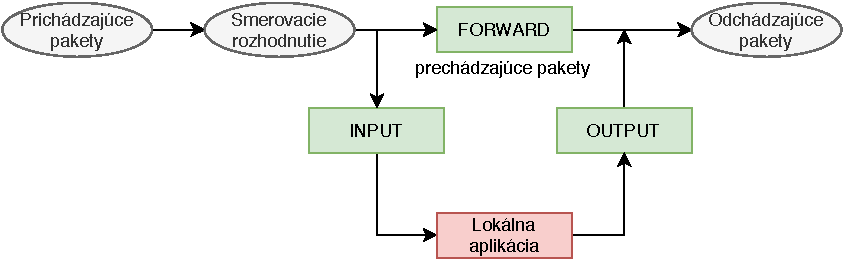
\includegraphics[scale=1.07]{obrazky-figures/iptables.pdf}
	\caption{Základné reťazce \emph{iptables} obsiahnuté v \emph{netfilteri} v tabuľke filter}
\end{figure}
                                                                                              
\emph{iptables} ponúka konfiguráciu \emph{netfilteru} ako stavového paketového filtra možného filtrovať sieťovú prevádzku na základe typu protokolu, zdrojovej a cieľovej adresy, zdrojového a cieľového portu, znalostí protokolu a ich stavoch. 

Hlavným problémom \emph{iptables} a dôvodom zlej reputácie, je primárne vysoká duplicita kódu, nakoľko existuje samostatná tabuľka pre každý sieťový protokol, problémy so škálovaním, rýchlosť spracovávania a mnohé iné.

\subsection{nftables}
\label{nftables}
Náhrada \emph{iptables} vo forme \emph{nftables} je podsystém v Linuxovom jadre, ktorý mení a nahradzuje určité časti samotného \emph{netfilteru}. Základným blokom tohto podsystému je pridanie virtuálneho stroja do Linuxového jadra, ktorý je schopný spúšťať binárny kód určený na prezeranie sieťových paketov a rozhodovanie podľa pravidiel \cite{manpages, netfilter}. 

                                                                                 
\emph{nftables} neobsaujú žiaden špecifický kód naviazaný na protokol a umožnujú analyzovať aj neznáme pakety, ktorých spracovanie je definované užívateľom cez userspace program \emph{nft}. V prípade nutnosti rozšírenia samotného firewallu je teda nutné len vytvoriť nový binárny kód, ktorý je následne vložený do virtuálneho stroja na vykonávanie a mimo toho nie je potreba meniť žiadnu časť jadra.

\chapter{Návrh aplikácie}
\label{app-design}

	V tejto kapitole sú popísané jednotlivé prvky firewall aplikácie, hlavne teda grafické prostredie 
	pre správu a analýzu, ale aj jadro samotného firewallu. Celý projekt je vyvinutý v jazyku \texttt{Python3.6},
	ktorý ponúka univerzálnosť, jednoduchosť a veľa možností, ktoré uľahčujú a zrýchľujú vývoj projektov.

	\section{Virtuálne prostredie}
	\label{pipenv}
		Celá aplikácia je vyvíjaná vo virtuálnom prostredí \texttt{pipenv}, aby bol zaručená zhoda verzií 
		jednotlivých externých modulov na rôznych systémoch, hlavne teda počas vývoja a nasadenia aplikácie
		na strane servera. Všetky potrebné balíky su definované aj s konkrétnymi verziami v súbore \texttt{Pipfile}.

	\section{Grafické rozhranie}
	\label{gui}
		Táto aplikácia je navrhnutá, aby bežala ako služba na servery, ktorý slúži ako firewall. Jedným
		z cieľov tohto projektu je, aby aplikácia poskytovala štatistiky vo forme grafov. Aby sme sa vyhli
		inštalácií grafického prostredia na firewalle, ktoré je závislé na množstve rôznych balíkov, rozhodli
		sme sa vytvoriť užívateľské rozhranie pomocou webového frameworku \texttt{Django} (popisaný v sekcií
		\ref{django}). Cez tento web bude možné upravovať konfiguráciu firewallu a sledovať aj dynamicky 
		generované grafy pomocou \texttt{HighCharts} (popísaný v sekcií \ref{highcharts}).

		\subsection{Django}
		\label{django}
			Webový framework \texttt{Django} je napísaný v jazyku \texttt{Python} a slúži na rýchly vývoj 
			a návrh aplikácií. Hlavnou myšlienkou je nevyvíjať už existujúce veci a riešenia, ale zamerať
			sa hlavne na novú aplikáciu. V základe každého \texttt{Django} projektu nájdeme autentifikáciu
			užívateľov a abstrakciu nad rôznymi databázovými systémami. Tento framework používa poupravený 
			\texttt{Jinja2} šablónovací systém pre generovanie html stránok \cite{django}.
		
		\subsection{HighCharts}
		\label{highcharts}
			Tento JavaScriptový modul slúži na generovanie veľkého množstva rôznych interaktívnych webových
			grafov ako napríklad čiarové, koláčové či pruhový graf. Práca s týmto modulom je veľmi jednoduchá
			a spočíva vo vytvorení reťazca dát vo formáte \texttt{JSON}, ktorý obsahuje všetky potrebné 
			informácie. O zvyšok sa uz modul postará sám \cite{highcharts}.
		        
	\section{Firewall}
		Tento firewall používa \texttt{nftables} na filtrovanie sieťovej trafiky. Konfigurácia môže byť 
		zadaná priamo pomocou programu \texttt{nft} alebo pomocou webového grafického rozhrania, kde je
		textové pole s aktuálnou konfiguráciou, ktorú možno upravovať. 

\chapter{Záver}

	Návrh aplikácie pre konfiguráciu firewall v systéme Linux je vyriešený a vďaka virtuálnemu prostrediu je schopná
	fungovať na rôznych Linuxových distribúciach. 
	
	Prototyp programu a webového rozhrania obhájil svoju vhodnosť ako riešenie daného problému a preto ostaneme pri 
	danom návrhu riešenia firewall aplikácie.
	
	V ďalšom kroku je nutné odladiť grafické rozhranie a overiť dáta z vygenerovaných grafov, či zodpovedajú a ukazujú
	správne údaje zo sond (čítače, \texttt{ntf} pravidlá).

	\section{Rozdelenie práce}
	
	\begin{itemize}
		\item Bc. Jozef Urbanovský <xurban66>
		\begin{itemize}
			\item firewall
			\item iptables
			\item nftables
		\end{itemize}
	
		\item Bc. Adrián Tomašov <xtomas32>
		\begin{itemize}
			\item Django
			\item HighCharts
			\item nftables sytntax a API
		\end{itemize}
		
	\end{itemize}
	

%=========================================================================
